\documentclass[a4paper,12pt,russian]{article} %draft
\usepackage[T2A]{fontenc}% Поддержка русских букв


% XeTeX packages
\usepackage[cm-default]{fontspec} % or install lmodern and remove cm-default opt
\usepackage{xunicode} % some extra unicode support
\usepackage{xltxtra} % \XeLaTeX macro


\tolerance=1000
\emergencystretch=0.74cm
\usepackage{indentfirst} %делать отступ в начале параграфа

\usepackage[pdfborder = {0 0 0}]{hyperref} %гиперссылки в документе.

\usepackage[utf8]{inputenc}	% кодировка текста
\usepackage[russian]{babel}	% руссификация по Бабелю
\usepackage{graphics}

\usepackage[clean,pdf]{svg}

\usepackage{amsmath, amsfonts} % для расширенных настроек ссылок на формулы
\usepackage{extsizes}	% использование шрифтов большего кегля 

\usepackage{fancyvrb} % Добавляет продвинутые Verbatim и Verb

\usepackage{epsfig} % удобно вставлять рисунки в строку текста
\usepackage[usenames,dvipsnames]{pstricks}
\usepackage{pst-grad} % For gradients
\usepackage{pst-plot} % For axes

\usepackage{graphicx,xcolor}

%\usepackage[MakeStamp]{eskdi}
%\usepackage[MakeStamp, SubSectInToc]{eskdi}
%\usepackage[MakeStamp, SubSubSectInToc]{eskdi}
%\usepackage[MakeStamp, ParagraphInToc]{eskdi}
%\usepackage[twoside, MakeStamp, ParagraphInToc]{eskdi}
%\usepackage{eskdi}
%\usepackage[SubSectInToc]{eskdi}
%\usepackage[SubSubSectInToc]{eskdi}
%\usepackage[ParagraphInToc]{eskdi}
%\usepackage[ParagraphInToc, NumIntoSections]{eskdi}
%\usepackage[twoside, ParagraphInToc]{eskdi}
%\usepackage[twoside, MakeEmptyStamp, ParagraphInToc]{eskdi}
\usepackage[twoside, MakeEmptyStamp]{eskdi}
%\usepackage[MakeEmptyStamp, ParagraphInToc]{eskdi}



\usepackage{array}
\usepackage{tabularx}
\usepackage{supertabular}
\usepackage{longtable} % для создания таблиц, переносящихся на другую страницу
%\usepackage{listingsutf8}%
\usepackage{listings} % для включения листинга кода в приложения. Русский язык глючит.


\lstloadlanguages{bash,[LaTeX]TeX,MetaPost,Clean,Matlab}


\usepackage{textcomp}	% Ввод различных знаков
\usepackage{keystroke} % для отображения символов клавиш
\usepackage{bytefield} %для создания таблиц с битовыми полями
\usepackage{filecontents} %для включения в документ содержимого файлов

\usepackage{tikz} % Пакет для рмсования диаграмм
\usepackage{tikz-timing}[2009/12/09]
\usetikzlibrary{positioning,arrows,automata,plotmarks} %В данном случае нам потребуются positioning и arrows, которые нужны для расположения элементов друг относительно друга и рисования стрелок между ними соответственно.
\usetikzlibrary{shapes,snakes}
\usepackage{schemabloc}

\usepackage{makecell} % Для многострочных ячеек таблицы
\usepackage{colortbl} % Для раскрашивания ячеек в таблицах


%{Arial} {Courier New} 
%{OpenGost Type A TT} {OpenGost Type B TT} % Свободный шрифт. Нет наклонного начертания и дирного начертания
%{GOST type A} % Морально устарел, не свободный, не хватает символа тирэ. Не рекомендуется
%{GOST type B} % Морально устарел, не свободный, не хватает символа тирэ. Не рекомендуется
\gostSetRomanfont{Times New Roman}%
\gostSetSansfont{Times New Roman}%
\gostSetMonofont{Times New Roman}%
\gostSetMainfont{Times New Roman}%
\gostSetStampfont{Arial}%


%\verbatimfont{\fontspec[Scale=1.0]{Arial} \itshape}% % Для замены стиля начертания verbatim и verb
\verbatimfont{\fontspec[Scale=1.0]{Consolas}}% % Для замены стиля начертания verbatim и verb
\newfontfamily{\gostListingfont}[Scale=1.0]{Consolas} % Шрифт для листингов
%\renewcommand{\SetStampfontIt}{\itshape}%

%\input commands.tex %Файл включает такие команды как надчёркивание, запрещение переноса ТУ и др.
\setpage % Разметка текста на странице
\begin{document}

	\gosttitleobject{Лабораторная работа}
		
	\gosttitledocument{КАНОНИЧЕСКИЕ ФОРМЫ ПРЕДСТАВЛЕНИЯ ДИНАМИЧЕСКИХ СИСТЕМ}

	% Раскомментировать если необходима утверждающая надпись на титульном листе
	\renewcommand\titleBotRIGHT{
	\spboxmm{100}{70}{70}{30}{lc}{\parbox{70mm}{
			\normalsize{Преподаватель: Чепинский С.А. }\\ 
			\normalsize{Студенты: Французов Р.А.\\  Донцова М.А.}\\
			\normalsize{Группа: R3325}\\
			\normalsize{Вариант: 18}}}}

		\maketitle
		
		\section{Цель работы}
		Ознакомление с методами взаимного перехода между моделями
		вход-выход и вход-состояние-выход, а также с каноническими формами представления
		моделей вход-состояние-выход. 
 \\
		
		\section{Ход работы}
Ниже представлены исходные данные варианта\\
\begin{center}
\begin{tabular}{|c|c|}
	\hline
	$a_0$ & 15
 \\ \hline
	$a_1$ & 5
 \\ \hline
	$a_2$ & 10
 \\ \hline
	$b_0$ & 15
 \\ \hline
	$b_1$ & 0.5
 \\ \hline
	$b_2$ & 1
 \\ \hline
\end{tabular}
\end{center}
и вход-состояние-выход\\
\begin{center}
	\begin{tabular}{|c|c|}
		\hline
		$A$ & 229.2
\\ \hline
		$B$ & ${\begin{pmatrix}2\cr 0\cr \end{pmatrix}}$
\\ \hline
		$C$ & ${\begin{pmatrix}2&1\cr \end{pmatrix}}$
 \\ \hline
		$M$ & ${\begin{pmatrix}5&0\cr 6&2\cr \end{pmatrix}}$
 \\ \hline
	\end{tabular}
\end{center}

\subsection{Переход от ВВ к ВСВ}
По исходным данным варианта составлено и упрощено уравнение для системы вход-выход:\\
$y^{(3)}+10\ddot{y}+5\dot{y}+15y=1\ddot{u}+0.5\dot{u}+15u$
\\
$s^3y+10s^2y+5sy+15y=1s^2u+0.5su+15u$
\\
из уравнений получена передаточная функция:\\
$W(s)=${\dfrac{15+0.5s+s^{2}}{15+5s+10s^{2}+s^{3}}}$
$\\
На основании коэффициентов передаточной функции составлены системы ВСВ в канонических управляемой и наблюдаемой формах:\\
$Aku=${\begin{pmatrix}0&1&0\cr 0&0&1\cr -15&-5&-10\cr \end{pmatrix}}$
;Bku=${\begin{pmatrix}0\cr 0\cr 1\cr \end{pmatrix}}$
;Cku=${\begin{pmatrix}15&0.5&1\cr \end{pmatrix}}$
$\\
$Akn=${\begin{pmatrix}0&0&-15\cr 1&0&-5\cr 0&1&-10\cr \end{pmatrix}}$
;Bkn=${\begin{pmatrix}15\cr 0.5\cr 1\cr \end{pmatrix}}$
;Ckn=${\begin{pmatrix}0&0&1\cr \end{pmatrix}}$
$\\
Составленные системы были промоделированы при единичном входном воздействии\\

\begin{figure}[H]
	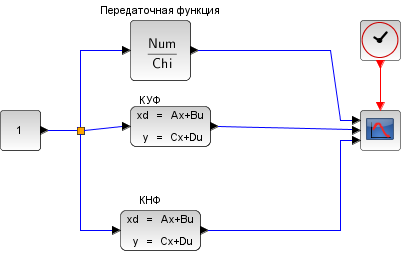
\includegraphics[width=0.7\textwidth]{tf}
	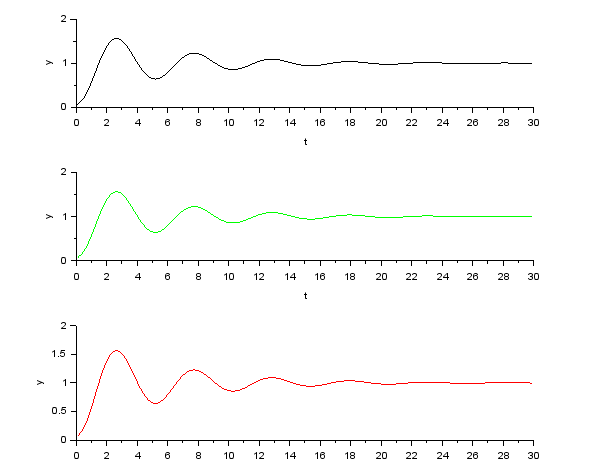
\includegraphics[width=1\textwidth]{tf-sim}
	\caption{Схема и результаты моделирования при единичном воздействии}
\end{figure}

\subsection{Переход от ВCВ к ВВ}
Использовано выражение для получения передаточной функции из начальной системы:\\
$W(s)=C(sI-A)^{-1}B={\begin{pmatrix}2&1\cr \end{pmatrix}}{\begin{pmatrix}-1+s&15\cr -1&3+s\cr \end{pmatrix}}^{-1}{\begin{pmatrix}2\cr 0\cr \end{pmatrix}}={\begin{pmatrix}2&1\cr \end{pmatrix}}{\begin{pmatrix}{\frac{3+1s}{12+2s+s^{2}}}&{\frac{-15}{12+2s+s^{2}}}\cr {\frac{1}{12+2s+s^{2}}}&{\frac{-1+1s}{12+2s+s^{2}}}\cr \end{pmatrix}}{\begin{pmatrix}2\cr 0\cr \end{pmatrix}}={\begin{pmatrix}{\frac{7+2s}{12+2s+s^{2}}}&{\frac{-31+1s}{12+2s+s^{2}}}\cr \end{pmatrix}}{\begin{pmatrix}2\cr 0\cr \end{pmatrix}}={\dfrac{14+4s}{12+2s+s^{2}}}
$\\

На основании коэффициентов передаточной функции составлены системы ВСВ в канонических управляемой и наблюдаемой формах:\\
$Aku=${\begin{pmatrix}0&1\cr -12&-2\cr \end{pmatrix}}$
;Bku=${\begin{pmatrix}0\cr 1\cr \end{pmatrix}}$
;Cku=${\begin{pmatrix}14&4\cr \end{pmatrix}}$
$\\
$Akn=${\begin{pmatrix}0&-12\cr 1&-2\cr \end{pmatrix}}$
;Bkn=${\begin{pmatrix}14\cr 4\cr \end{pmatrix}}$
;Ckn=${\begin{pmatrix}0&1\cr \end{pmatrix}}$
$\\

Составленные системы были промоделированы при единичном входном воздействии\\
\begin{figure}[H]
	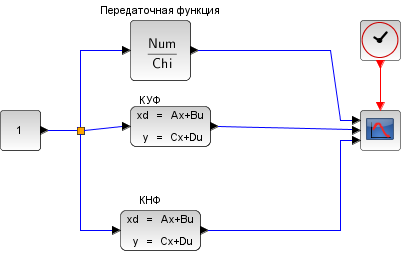
\includegraphics[width=0.7\textwidth]{SS}
	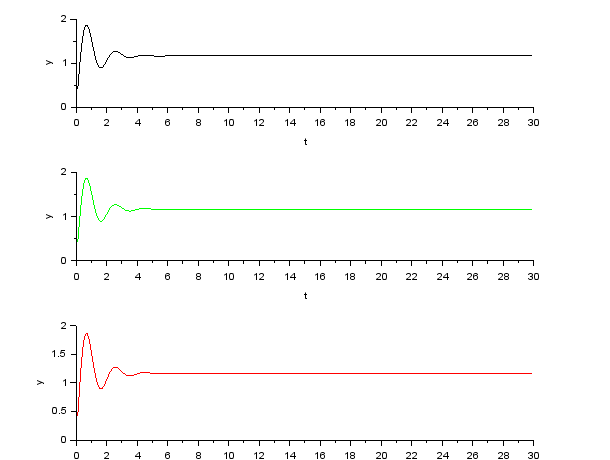
\includegraphics[width=1\textwidth]{SS-sim}
	\caption{Схема и результаты моделирования при единичном воздействии}
\end{figure}

Составленны матрицы управляемости для каждой системы $N=\begin{pmatrix}A & A*B\end{pmatrix}$:\\
$N=${\begin{pmatrix}2&2\cr 0&2\cr \end{pmatrix}}$
\\
Nku=${\begin{pmatrix}0&1\cr 1&-2\cr \end{pmatrix}}$
\\
Nkn=${\begin{pmatrix}14&-48\cr 4&6\cr \end{pmatrix}}$
$\\
Составлены матрицы преобразования для КУФ и КНФ $M=N \hat{N}^{-1}$:\\
$Mku=${\begin{pmatrix}6&2\cr 2&0\cr \end{pmatrix}}$
\\
Mkn=${\begin{pmatrix}0.014&0.449\cr -0.029&0.101\cr \end{pmatrix}}$
$\\

\subsection{Замена базиса в пространстве состояний}
С помощью формул была получена система, подобная начальной:\\
$\hat{A}=M^{-1}AM=${\begin{pmatrix}-17&-6\cr 44.5&15\cr \end{pmatrix}}$
\\
 \hat{B}=M^{-1}B=${\begin{pmatrix}0.4\cr -1.2\cr \end{pmatrix}}$
\\
 \hat{C}=CM=${\begin{pmatrix}16&2\cr \end{pmatrix}}$
$\\ 
 Обе системы были промоделированы при единичном входном воздействии:\\

\begin{figure}[H]
	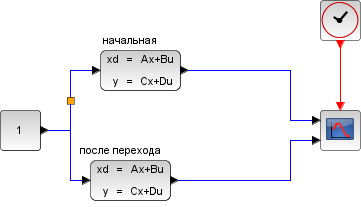
\includegraphics[width=0.7\textwidth]{change}
	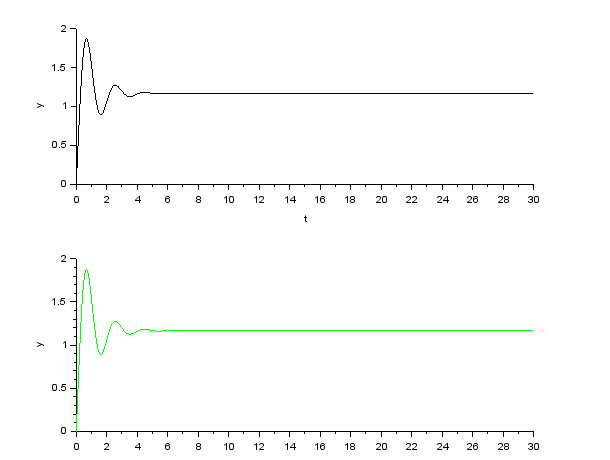
\includegraphics[width=1\textwidth]{change-sim}
	\caption{Схема и результаты моделирования при единичном воздействии}
\end{figure}


\section{Вывод}
В данной лабораторной работе был успешно совершен переход между системи вход-выход и вход-состояние-выход, переходные процессы систем, заданных в КУФ, КНФ и передаточной функцией, совпадают. Также успешно совершена смена базиса в пространстве состояний, в результате чего была получена подобная система, переходный процесс которой не отличается от начальной.
\end{document}